In the preliminaries we have seen how parity games can be used to verify if a modal $\mu$-calculus formula is satisfied by an LTS. Such a parity game contains the information needed to answer the question if an LTS satisfies a  modal $\mu$-calculus formula. We have also seen how an LTS can be extended with transition guards to model the behaviour of multiple LTSs. In this section we introduce \textit{variability parity games} (VPGs); a VPG extends the definition of a parity game much like an FTS extends the definition of an LTS. Similar as to how an FTS expresses multiple LTSs does a VPG express multiple parity games, moreover we introduce a way of creating VPGs such that every parity game it expresses contains the information needed to answer the question if a product in an FTS satisfies a modal $\mu$-calculus formula.

We extend parity games such that edges in the game are guarded. Instead of using features, feature expressions and products we choose a syntactically simpler representation and introduce \textit{configurations}. A VPG has a set of configurations and is played for a single configuration. Edges are guarded by sets of configurations; if the VPG is played for a configuration that is in the guard set then the edge is enabled, otherwise it is disabled.

\begin{definition}
	\label{def_VPG}
	A variability parity game (VPG) is a tuple $(V,V_0, V_1, E, \Omega, \mathfrak{C}, \theta)$, where:
	\begin{itemize}
		\item $V$,$V_0$,$V_1$, $E$ and $\Omega$ are defined as in parity games,
		\item $\mathfrak{C}$ is a non-empty finite set of configurations,
		\item $\theta : E \rightarrow 2^\mathfrak{C}\ \backslash\ \emptyset$ is a total function mapping every edge to a set of configurations guarding that edge.
	\end{itemize}
\end{definition}
VPGs are considered total when every vertex has at least one outgoing edge. Since edges are guarded with sets of configurations we also require that for every configuration $c \in \mathfrak{C}$ every vertex has at least one outgoing edge that admits configuration $c$, formally a VPG is total if and only if for all $v \in V$:
\[ \bigcup\{\theta(v,w)\ |\ (v,w) \in E\} = \mathfrak{C} \]

VPGs are depicted as parity games with labelled edges that represent the sets of configurations guarding them.

\begin{example}
	Figure \ref{fig:vpg_basicex} shows an example of a VPG with configuration $\mathfrak{C} = \{c_0,c_1,c_2\}$.
	\begin{figure}[h]
		\centering
		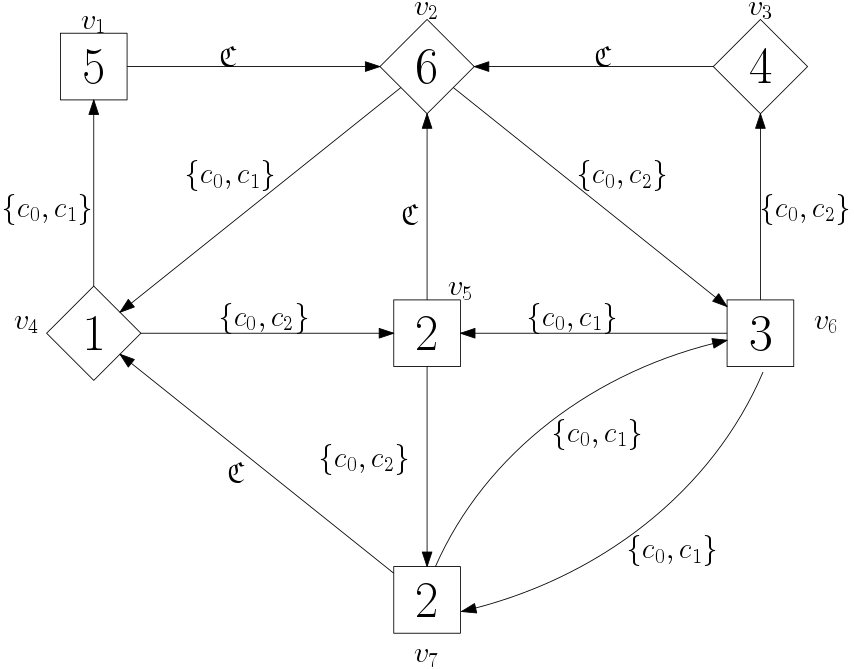
\includegraphics[scale=0.3]{Examples/VPG/Basic}
		\caption{VPG with configurations $\mathfrak{C} = \{c_0,c_1,c_2\}$}
		\label{fig:vpg_basicex}
	\end{figure}
\end{example}

A VPG can be played for a vertex-configuration pair. When playing a VPG for $v\in V$ and $c \in \mathfrak{C}$ we start by placing a token on vertex $v$. We proceed with the game similar as with a parity game however player $\alpha$ can only move the token from $v \in V_\alpha$ to $w \in V$ if $(v,w) \in E$ and $c \in \theta(v,w)$. Similar as in a parity game this results in a path. Again the winner is determined by the highest priority occurring infinitely often in the path or, in case of a finite path, the winner is the opponent of the player that can't make a move any more. Paths might be valid for some configurations but not valid for others, we call a path valid for configuration $c$ if and only if for every $i > 0$ we get $(\pi_{i},\pi_{i+1}) \in E$ and $c \in \theta(\pi_{i},\pi_{i+1})$.

Moves made by the players can again be determined by strategies, however for different configurations for which the game is played different strategies might be needed. So we define a strategy not only for a player but also for a configuration. We define a strategy for player $\alpha$ and configuration $c \in \mathfrak{C}$ as a partial function $\sigma_\alpha^c : V^*V_\alpha \rightarrow V$ that maps a series of vertices ending with a vertex owned by player $\alpha$ to the next vertex such that for any $\sigma_\alpha^c(w_0\dots w_m) = w$ we have $(w_m,w) \in E$ and $c \in \theta(w_m,w)$. A path $\pi$ conforms to strategy $\sigma_\alpha^c$ if for every $i > 0$ with $\pi_{i-1}\in V_\alpha$ we have $\pi_i = \sigma_\alpha(\pi_0\pi_1\dots\pi_{i-1})$.

A strategy is winning in configuration $c$ for player $\alpha$ from vertex $v$ if and only if $\alpha$ is the winner of every valid path for $c$ starting in $v$ that conforms to $\sigma_\alpha$.

\begin{example}
	Consider the VPG in Figure \ref{fig:vpg_basicex}. When playing the game for vertex $v_5$ and configuration $c_0$ we can define strategy 
	\[ \sigma_1^{c_0} = \{ v_5 \mapsto v_7, v_7\mapsto v_6,v_6\mapsto v_7, \dots \}\]
	This always results in the path $v_5(v_7v_6)\omega$ where the highest priority occurring infinitely often is 3 so player 1 wins. Since this is the only valid path vertex $v_5$ is won by player 1 in configuration $c_0$.
	
	If the game is played for vertex $v_5$ and configuration $c_1$ the strategy $\sigma_1^{c_0}$ is not valid because the edge $(v_5,v_7)$ is not enabled. For player $0$ we can define strategy
	\[ \sigma_0^{c_1} = \{ v_2 \mapsto v_4, v_4 \mapsto v_1,\dots\}\]
	Player 1 can only play from $v_5$ to $v_2$ so the only path that conforms to $\sigma_0^{c_1}$ is $v_5(v_2v_4v_1)^\omega$ which is winning for player 0. So vertex $v_5$ is won by player 0 in configuration $c_1$.
	
	When playing the game for vertex $v_5$ and configuration $c_2$ the we use the same strategy as used in configuration $c_1$, we get $\sigma_1^{c_2} = \sigma_1^{c_0}$ and vertex $v_5$ is winning for player 1 in configuration $c_2$.
\end{example}

A VPG is solved if for every configuration $c$ the vertices are partitioned in two sets, namely $W_0^c$ and $W_1^c$, such that every vertex in $W_\alpha^c$ is winning for player $\alpha$ in configuration $c$. We call these sets the winning sets of a VPG.

We can create a parity game from a VPG by simply choosing configuration $c$ and removing all the edges that do not have $c$ in their guard set. We call this a projection.

\begin{definition}
	\label{def_vpg_proj}
	The projection of VPG $G = (V,V_0,V_1,E,\Omega, \mathfrak{C},\theta)$ onto configuration $c\in \mathfrak{C}$, denoted by $G_{|c}$, is the parity game $(V,V_0,V_1,E',\Omega)$ where $E' = \{ e \in E\ |\ c \in \theta(e)\}$.
\end{definition}
If a VPG is total then there is at least one outging edge for every vertex that admits configuration $c \in \mathfrak{C}$. This edge will be in the projection $G_{|c}$ so clearly when the VPG is total then its projections are also total.

A VPG contains multiple parity games, in fact playing a VPG $G$ for configuration $c$ is the same as playing the parity game $G_{|c}$ which we show in the following lemma's and theorem.

\begin{lemma}
	\label{lem_path_in_VPG_valid_iff_path_in_proj_valid}
	Path $\pi$ is valid in $G = (V,V_0,V_1,E,\Omega,\mathfrak{C},\theta)$ for configuration $c$ if and only if path $\pi$ is valid in $G_{|c} = (V,V_0,V_1,E',\Omega)$.
	\begin{proof}
		Consider path $\pi$ that is valid in $G$ for configuration $c$. For every $i>0$ we have $(\pi_{i-1},\pi_i) \in E$ and $c \in \theta(\pi_{i-1},\pi_i)$. Using the projection definition (Definition \ref{def_vpg_proj}) we can conclude that $(\pi_{i-1},\pi_1) \in E'$ making the path valid in $G_{|c}$.
		
		Consider path $\pi$ that is valid in $G_{|c}$. For every $i > 0$ we have $(\pi_{i-1},\pi_i) \in E'$. Given the projection definition we find that because $(\pi_{i-1},\pi_i) \in E'$ we must have $(\pi_{i-1},\pi_i) \in E$ and $c \in \theta(\pi_{i-1},\pi_i)$. This makes the path valid in $G$ for configuration $c$.
	\end{proof}
\end{lemma}

\begin{lemma}
	\label{lem_start_in_VPG_valid_iff_start_in_proj_valid}
	Any strategy $\sigma_\alpha^c$ for player $\alpha$ and configuration $c \in \mathfrak{C}$ in VPG $G = (V,V_0,V_1,E,\Omega,\mathfrak{C},\theta)$ is also a strategy in $G_{|c}$ for player $\alpha$ and any strategy $\sigma_\alpha$ for player $\alpha$ in $G_{|c}$ is also a strategy in $G$ for player $\alpha$ and configuration $c$.
	\begin{proof}
		The exact same reasoning as in lemma \ref{lem_path_in_VPG_valid_iff_path_in_proj_valid} can be applied to prove this lemma.
	\end{proof}
\end{lemma}

\begin{theorem}
	\label{the_winning_set_is_equal_to_proj_winning_set}
	Winning sets $(W_0^c, W_1^c)$ of VPG $G = (V,V_0,V_1,E,\Omega,\mathfrak{C},\theta)$ played for configuration $c \in \mathfrak{C}$ are equal to winning sets $(Q_0,Q_1)$ of parity game $G_{|c}$.
	\begin{proof}
		Let $v \in W_\alpha^c$ for some $\alpha \in \{0,1\}$. There exists a strategy $\sigma_\alpha^c$ in VPG $G$ for player $\alpha$ and configuration $c$ such that any valid path starting in $v$ is winning for player $\alpha$. As shown in lemma \ref{lem_start_in_VPG_valid_iff_start_in_proj_valid}, $\sigma_\alpha^c$ is also a strategy for player $\alpha$ in $G_{|c}$. Any valid path starting in $v$ in game $G$ played for configuration $c$ is also valid in game $G$ as shown in lemma \ref{lem_path_in_VPG_valid_iff_path_in_proj_valid}, additionally any path valid in $G_{|c}$ is also valid in $G$ played for $c$. Assume there is a valid path in $G_{|c}$ that conforms to $\sigma_\alpha^c$ starting from $v$ that is not won by player $\alpha$. This path is also valid in $G$ played for configuration $c$ which contradicts $v \in W_\alpha^c$, therefore no such path exists and strategy $\sigma_\alpha^c$ is winning for player $\alpha$ from $v$ in parity game $G_{|c}$, hence $v \in Q_\alpha$.
		
		Let $v \in Q_\alpha$ for some $\alpha \in \{0,1\}$. There exists a strategy $\sigma_\alpha$ in parity game $G_{|c}$ for player $\alpha$ such that any valid path starting in $v$ is winning for player $\alpha$. Using lemma \ref{lem_start_in_VPG_valid_iff_start_in_proj_valid} we find that $\sigma_\alpha$ is a strategy in game $G$ for player $\alpha$ and configuration $c$. Assume there is a valid path in $G$ for $c$ that conforms to $\sigma_\alpha$ starting from $v$ that is not won by player $\alpha$. This path is also valid in $G_{|c}$ which contradicts $v \in Q_\alpha$, therefore no such path exists and strategy $\sigma_\alpha$ is winning for player $\alpha$ and configuration $c$ from $v$ in VPG $G$, hence $v \in W_\alpha^c$.
	\end{proof}
\end{theorem}

Parity games have a unique winner for every vertex, from theorem \ref{the_winning_set_is_equal_to_proj_winning_set} we can conclude that a VPG player for a configuration also has a unique winner for every vertex. Moreover since it is decidable who wins a vertex in a parity game it is also decidable who wins a vertex in a VPG for configuration $c$. Finally, in a parity game there exists a positional strategy for player $\alpha$ that is winning for all the vertices won by player $\alpha$ in the game. In theorem \ref{the_winning_set_is_equal_to_proj_winning_set} we argued that a strategy that is winning for player $\alpha$ starting in vertex $v$ in a projection of $G$ onto $c$ is also winning in $G$ for player $\alpha$ and configuration $c$ starting in vertex $v$. So we can conclude that VPGs are also positionally determined and we can consider a strategy for player $\alpha$ and configuration $c$ as a total function $\sigma_\alpha^c : V_\alpha \rightarrow V$.

\subsection{Verifying featured transition systems}
Given an LTS and a modal $\mu$-calculus formula we can construct a parity game such that solving this parity game tells us if the LTS satisfies the formula. Similarly we can construct a VPG from an FTS and a modal $\mu$-calculus in such a way that solving the VPG tells us what products satisfy the formula.

We create a VPG from an FTS by choosing the set of configurations to be equal to the set of products in the FTS. The game graph is created similar as to how a parity game is created from an LTS. Finally we guard edges going from vertices representing a modal formula.

\begin{definition}
	\label{def_FTS2VPG}
	FTS2VPG($M, \varphi$) converts FTS $M = (S, Act, trans, s_0, N, P, \gamma)$ and closed formula $\varphi$ to VPG $(V, V_0, V_1, E, \Omega, \mathfrak{C},\theta)$.
	
	The set of configurations is equal to the set of products, ie. $\mathfrak{C} = P$.
	
	Vertices are created for every state with every formula in the Fischer-Ladner closure of $\varphi$. We define the set of vertices:
	\[ V = (S \times \textit{FL}(\varphi))\]
	
	The following table shows the owner, successors and edge guards of vertices where we write $w\ |\ C$ as a successor of $v$ to denote that there is an edge $(v,w) \in E$ such that the edge is guarded by set $C \subseteq \mathfrak{C}$, i.e. $\theta(v,w) = C$. 
	\begin{center}
		\begin{tabular}{l|l|l}
			Vertex & Owner & Successor$\ |\ $ guard set \\\hline
			$(s,\bot)$ & 0     &        \\
			$(s,\top)$ & 1     &        \\
			$(s,\psi_1 \vee \psi_2)$ & 0       & $(s,\psi_1)\ |\ \mathfrak{C}$ and $(s,\psi_2)\ |\ \mathfrak{C}$ \\
			$(s,\psi_1 \wedge \psi_2)$ & 1       & $(s,\psi_1)\ |\ \mathfrak{C}$ and $(s,\psi_2)\ |\ \mathfrak{C}$ \\
			$(s, \langle a \rangle \psi)$ & 0 & $(s',\psi)\ |\ \{c \in \mathfrak{C}\ |\ c \models g\}$ for every $s \xrightarrow{ a\ |\ g} s'$\\
			$(s, [ a ] \psi)$ & 1 & $(s',\psi)\ |\ \{c \in \mathfrak{C}\ |\ c \models g\}$ for every $s \xrightarrow{ a\ |\ g} s'$\\
			$(s, \mu X. \psi)$ & 1 & $(s, \psi[X:= \mu X. \psi])\ |\ \mathfrak{C}$ \\
			$(s, \nu X. \psi)$ & 1 & $(s, \psi[X:= \nu X. \psi])\ |\ \mathfrak{C}$ 
		\end{tabular}
	\end{center}
	
	Since the Fischer-Ladner formula's are closed we never get a vertex $(s,X)$.
	
	Finally we have $\Omega(v) = \begin{cases}
	2 \lfloor adepth(X) / 2 \rfloor & \text{if } v = (s,\nu X. \psi)\\
	2 \lfloor adepth(X) / 2 \rfloor + 1 & \text{if } v = (s,\mu X. \psi)\\
	0 & \text{otherwise}
	\end{cases}$
\end{definition}
Similar to parity games a VPG can be made total by creating sink vertices $l_0$ and $l_1$ with priority 1 and 0 respectively and each having an edge to itself with guard set $\mathfrak{C}$. When the VPG is played for configuration $c$ and the token ends up in $l_\alpha$ then clearly player $\alpha$ looses. We make a VPG total by adding vertices $l_0$ and $l_1$ and adding an edge from every vertex $v \in V_\alpha$ that has $\bigcup \{ \theta(v,w)\ |\ (v,w) \in E \} \neq \mathfrak{C}$ to $l_\alpha$ with guard set $\mathfrak{C} \backslash \bigcup \{ \theta(v,w)\ |\ (v,w) \in E \}$. Any vertex $v_\alpha$ where player $\alpha$ could not have made a move in the original game played for configuration $c$ now has an edge admitting $c$ to $l_\alpha$ where player $\alpha$ still looses. An edge admitting $c$ is only added if there was no outgoing edge admitting $c$ so the winner of vertex $v$ for configuration $c$ in the original game is the same as in the total game.

\begin{example}
	\label{ex_FTS2VPG}
	Consider FTS $M$ as shown in Figure \ref{fig:exverfts} that has features $f$ and $g$ and products $\{\emptyset,\{f\},\{f,g\}\}$. Modal $\mu$-calculus formula $\varphi = \mu X.([a]X \vee \langle b \rangle \top)$ expresses that on any path reached by \textit{a}'s we can eventually do a \text{b} action. This holds true for product $\{\emptyset\}$ because $s_1$ can only go to $s_2$ where $b$ can always be done. For product $\{f\}$ this doesn't hold because ones in $s_1$ it is possible to stay in $s_1$ indefinitely through an $a$ transition. For product $\{f,g\}$ however the formula does hold because we can indeed stay in $s_1$ indefinitely however from $s_1$ we can always do a $b$ step.
	
	
	Figure \ref{fig:exvevpg} shows the VPG resulting from \textit{FTS2VPG}$(M,\varphi)$ made total using sink vertices $l_0$ and $l_1$. Products $\{\emptyset\},\{f\},\{f,g\}$ are depicted as configurations $c_0,c_1,c_2$ respectively.
	\begin{figure}[h]
		\centering
		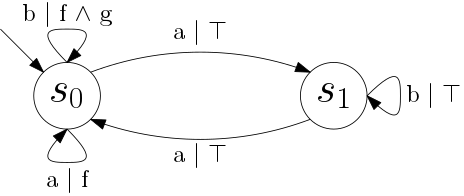
\includegraphics[scale=0.3]{Examples/ExamleVerification/FTS}
		\caption[FTS $M$]{FTS $M$}
		\label{fig:exverfts}
	\end{figure}
	\begin{figure}[h]
		\centering
		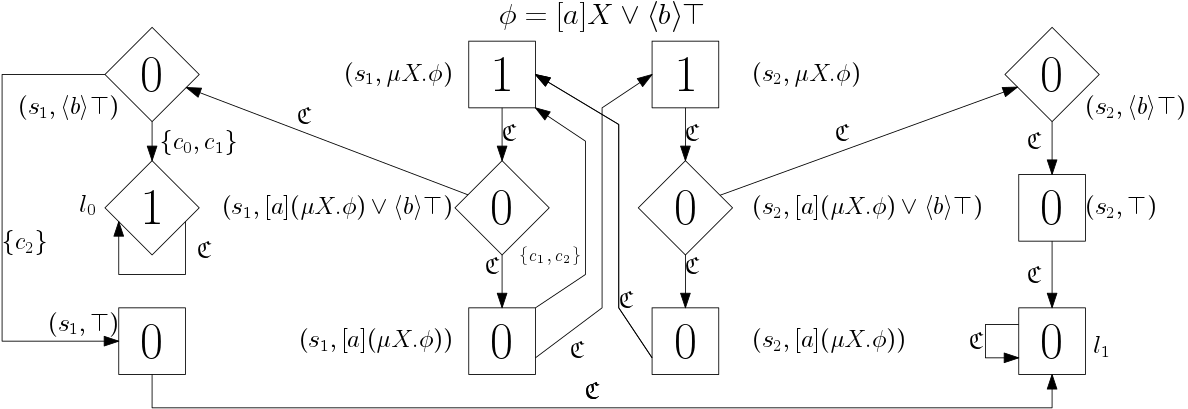
\includegraphics[scale=0.3]{Examples/ExamleVerification/VPG}
		\caption[VPG]{Total VPG created by \textit{FTS2VPG}}
		\label{fig:exvevpg}
	\end{figure}	
\end{example}

In order to prove that solving a VPG created by \textit{FTS2VPG} can be used to model check an FTS we inspect the relations we have seen between FTSs, LTSs, parity games and VPGs. Given FTS $M$ and formula $\varphi$ we can project $M$ onto a product to create an LTS and create a parity game from the resulting LTS and $\varphi$ using \textit{LTS2PG}. Alternatively we can create a VPG from $M$ and $\varphi$ using \textit{FTS2VPG} which can be projected onto a configuration to get a parity game. These different transformations are shown in the following diagram, where $\Pi_p$ depicts a projection onto product $p$ or configuration $p$:\\
\begin{tikzpicture}
\matrix (m) [matrix of math nodes,row sep=4em,column sep=1em,minimum width=2em]
{
	\text{\ \ FTS }M & \  & \ &\ & \text{VPG } \hat{G}  \\
	\text{LTS }M_{|p} & \ & \ & \text{PG } G & \text{\ \ PG }\hat{G}_{|p} \\};
\path[-stealth]
(m-1-1) edge [double] node [left] {$\Pi_p$} (m-2-1)
edge node [above] {\textit{FTS2VPG}$(M,\varphi)$} (m-1-5)
(m-2-1.east|-m-2-4) edge node [above] {\textit{LTS2PG}$(M_{|p},\varphi)$}
(m-2-4)
(m-1-5) edge [double] node [right] {$\Pi_p$} (m-2-5);
\end{tikzpicture}\\
In the following lemma we prove that in fact parity game $G$ and $\hat{G}_{|p}$ are identical.
\begin{lemma}
	\label{lem_VPG_proj_is_FTS_proj}
	Given FTS $M = (S, Act, trans, s_0, N, P, \gamma)$, closed modal $\mu$-calculus formula $\varphi$ and product $p \in P$ it holds that parity games LTS2PG$(M_{|p}, \varphi)$ and FTS2VPG$(M, \varphi)_{|p}$ are identical.
	\begin{proof}
		Let $\hat{G} = (\hat{V},\hat{V}_0,\hat{V}_1,\hat{E},\hat{\Omega},\mathfrak{C},\theta)$ be the VPG created from \textit{FTS2VPG}$(M,\varphi)$ and let $G = (V,V_0,V_1,E,\Omega)$ be the parity game created from \textit{LTS2PG}$(M_{|p},\varphi)$. Let the projection of $\hat{G}$ onto $p$ (using Definition \ref{def_vpg_proj}) be the parity game $G_{|p} = (\hat{V},\hat{V}_0,\hat{V}_1,\hat{E}',\hat{\Omega})$. We will prove that $\hat{G}_{|p} = G$.
		
		First observe that when an FTS is projected onto a product (using Definition \ref{def_fts_proj}) the FTS has the same states as the projection, we find that FTS $M$ has the same states as $M_{|p}$. The vertices created by \textit{LTS2PG} and \textit{FTS2VPG} rely only on the formula and the states in the LTS and FTS respectively. Similarly the owner and priority of these vertices is only determined by the states and the formula. Given that $M$ and $M_{|p}$ have the same states we find that $\hat{V} = V$, $\hat{V}_0 = V_0$, $\hat{V}_1 = V_1$ and $\hat{\Omega} = \Omega$.
		
		We are left with showing $\hat{E}' = E$ in order to conclude $\hat{G}_{|p} = G$. Consider vertex $v$, we distinguish two cases. 
		
		Let $v = (s,\langle a \rangle \psi)$ or $v = (s,[a] \psi)$. If $v$ has a successor to $(s',\psi)$ in $G$ then we have $s \xrightarrow{a} s'$ in $M_{|p}$ and therefore $s \xrightarrow{a\ |\ f} s'$ with $p \models f$ in $M$. Using the \textit{FTS2VPG} definition we find that vertex $v$ in $\hat{G}$ has successor $(s',\psi)$ with a guard containing $p$. Since $p$ is in the guard set we also find this successor in the projection $\hat{G}_{|p}$. 
		
		If $v$ has a successor to $(s',\psi)$ in $\hat{G}_{|p}$ then in $\hat{G}$ the edge from $v$ to $(s',\psi)$ also exists and the set guarding it contains $p$. In $M$ we find $s \xrightarrow{a\ |\ g} s'$ with $p \models g$, therefore we find $s \xrightarrow{a} s'$ in $M_{|p}$. Using the \textit{LTS2PG} definition we find that vertex $v$ in $G$ has successor $(s',\psi)$.
		
		Let $v \neq (s,\langle a \rangle \psi)$ and $v \neq (s,[a]\psi)$. Any successor of $v$ created by \textit{LTS2PG} does not depend on the LTS but only on the formula. Similarly any successor of $v$ created by \textit{FTS2VPG} does not depend on the FTS and has guard set $\mathfrak{C}$. The two definitions create the same successors for $v$ so the successors in games $G$ and $\hat{G}$ are the same. Since the guard sets of these successors are always $\mathfrak{C}$ the successors are also the same in $\hat{G}_{|p}$.
		
		We have proven $\hat{E}' = E$ and therefore $\hat{G}_{|p} = G$.
	\end{proof}
\end{lemma}
Using this Lemma we get the following diagram showing the relation between FTSs, LTSs, parity games and VPGs.\\
\begin{tikzpicture}
\matrix (m) [matrix of math nodes,row sep=4em,column sep=1em,minimum width=2em]
{
	\text{\ \ FTS }M & \  & \ &\ & \text{VPG } \hat{G}  \\
	\text{LTS }M_{|p} & \ & \ & \  & \text{\ \ PG }\hat{G}_{|p} \\};
\path[-stealth]
(m-1-1) edge [double] node [left] {$\Pi_p$} (m-2-1)
edge node [above] {\textit{FTS2VPG}$(M,\varphi)$} (m-1-5)
(m-2-1.east|-m-2-5) edge node [above] {\textit{LTS2PG}$(M_{|p},\varphi)$}
(m-2-5)
(m-1-5) edge [double] node [right] {$\Pi_p$} (m-2-5);
\end{tikzpicture}\\
We know from existing theory that solving a parity game constructed using \textit{LTS2PG} can be used to model check an LTS, furthermore we have seen that the winning sets of an VPG for configuration $c$ are equal to the winning sets of that VPG projected onto $c$. Given these facts and the lemma above we can prove that VPGs can be used to model check FTSs.
\begin{theorem}
	\label{the_FTS2VPG_is_correct} Given:
	\begin{itemize}
		\item FTS $M = (S,Act,trans,s_0,N,P,\gamma)$,
		\item closed modal $\mu$-calculus formula $\varphi$,
		\item product $p \in P$ and
		\item state $s \in S$
	\end{itemize}
it holds that $(M_{|p},s) \models \varphi$ if and only if $(s,\varphi) \in W_0^p$ in FTS2VPG$(M,\varphi)$.
\begin{proof}
	Assume $(M_{|p},s) \models \varphi$, using the relation between LTSs and parity games (Theorem \ref{the_LTS_PG_REL}) we find that vertex $(s_0,\varphi)$ in parity game \textit{LTS2PG}$(M_{|p},\varphi)$ is won by player 0. Using Lemma \ref{lem_VPG_proj_is_FTS_proj} we find that vertex $(s_0,\varphi)$ is also in game \textit{FTS2VPG}$(M,\varphi)_{|p}$ and is also won by player 0. Using Theorem \ref{the_winning_set_is_equal_to_proj_winning_set} we find that the winning sets of a VPG for configuration $c$ are the same as the winning sets of the projection of the VPG onto $c$. We find that vertex $(s_0,\varphi)$ is winning in game \textit{FTS2VPG}$(M,\varphi)$ for configuration $p$, hence $(s,\varphi) \in W_0^p$.
	
	Similarly if $(M_{|p},s) \not\models \varphi$ vertex $(s_0,\varphi)$ is won by player 1 in parity game \textit{LTS2PG}$(M_{|p},\varphi)$ and we get $(s,\varphi) \notin W_0^p$.
\end{proof}
\end{theorem}

\begin{example}
	Again consider Example \ref{ex_FTS2VPG}. We argued that $M$ satisfies $\varphi$ for products $\{\emptyset\}$ and $\{f,g\}$. We see that in VPG in Figure \ref{fig:exvevpg} that $(s_1,\mu X.([a]X \vee \langle b \rangle \top))$ is indeed winning for player 0 when played for $\{\emptyset\} = c_0$ using the strategy
	\[ \sigma_0^{c_0} = \{ (s_1,[a](\mu X. \phi) \vee \langle b \rangle \top) \mapsto (s_1,[a](\mu X.\phi)) , (s_2,[a](\mu X.\phi)\vee \langle b \rangle \top) \mapsto (s_2,\langle b \rangle \top ),\dots \}\]
	Using this strategy play always ends up in $l_1$ which is winning for player 0.
	
	For product $\{f\} = c_1$ player $1$ wins using strategy
	\[ \sigma_1^{c_1} = \{ (s_1,[a](\mu X. \phi)) \mapsto (s_1,\mu X.\psi),\dots \}\]
	Using this strategy we either infinitely often visit $(s_1,\mu X.\psi)$ in which case player 1 wins or player 0 can decide to play to $(s_1,\langle b \rangle \top)$ in which case play ends in $l_0$ and player 1 wins.
	
	For product $\{f,g\} = c_2$ player 0 wins using strategy
	\[ \sigma_0^{c_2} = \{ (s_1,[a](\mu X. \phi) \vee \langle b \rangle \top) \mapsto (s_1,\langle b \rangle \top), (s_1, \langle b \rangle \top) \mapsto (s_1,\top),\dots \}\]
	Using this strategy player 0 can prevent the path infinitely often visiting $(s_1,\mu X.\psi)$ by playing to $(s_1,\langle b \rangle \top)$ and to $(s_1,\top)$ next which brings the play in $l_1$ winning it for player 0.
\end{example}

We conclude by showing visualizing the verification of an FTS in figure \ref{fig:ftsverificationusingvpg}.
\begin{figure}[h]
	\centering
	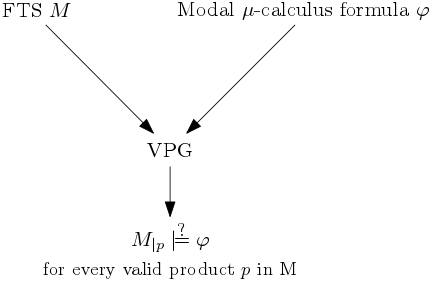
\includegraphics[scale=0.5]{Diagrams/FTSVerificationUsingVPG}
	\caption[FTS verification using VPG]{FTS verification using VPG}
	\label{fig:ftsverificationusingvpg}
\end{figure}